\section{Introduction:}

A popular method for converting an analog voltage into a digital value is the dual-slope method. Figure 1.0 {\bfseries (a)} shows a block diagram of the basic dual-slope converter. The analog voltage to be converted is applied through an electronic switch to an integrator or ramp-generator circuit (essentially a constant current charging a capacitor to produce a linear ramp voltage). The digital output is obtained from a counter operated during both positive and negative slope intervals of the integrator. The method of conversion proceeds as follows. For a fixed time interval (usually the full count range of the counter), the analog voltage connected to the integrator raises the voltage at the comparator input to some positive level. Figure 1.0 {\bfseries (b)} shows that at the end of the fixed time interval the voltage from the integrator is greater for the larger input voltage. At the end of the fixed count interval, the count is set to zero and the electronic switch connects the integrator to a reference or fixed input voltage. \hfill \break

\begin{figure}[H]
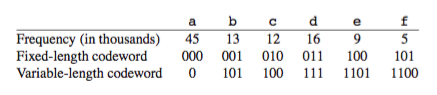
\includegraphics[height = 6cm, width = 16.5cm]{1.png}
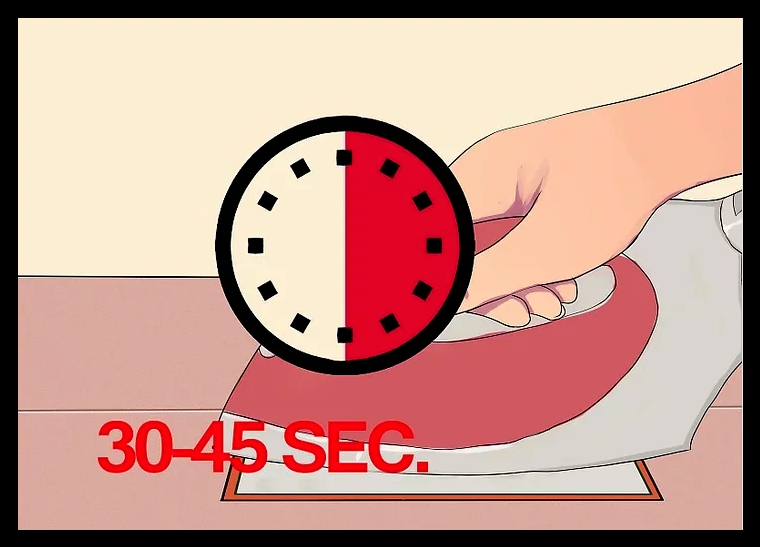
\includegraphics[height = 6cm, width = 16.5cm]{2.png}
\centering \linebreak \linebreak {\small Figure 1.0: Analog-to-digital conversion using dual-slope method: (a) logic diagram; (b) waveform}
\end{figure} \hfill \break

The integrator output (or capacitor input) then decreases at a fixed rate. The counter advances during this time, while the integrator’s output decreases at a fixed rate until it drops below the comparator reference voltage, at which time the control logic receives a signal (the comparator output) to stop the count. The digital value stored in the counter is then the digital output of the converter. Using the same clock and integrator to perform the conversion during positive and negative slope intervals tends to compensate for clock frequency drift and integrator accuracy limitations. Setting the reference input value and clock rate can scale the counter output as desired. The counter can be a binary, BCD, or other form of digital counter, if desired. 

\pagebreak

\subsection{Ladder-Network Conversion:}

Another popular method of analog-to-digital conversion uses a ladder network along with counter and comparator circuits ( see Figure 1.1 ). A digital counter advances from a zero count while a ladder network driven by the counter outputs a stair- case voltage, as shown in Figure 1.1 {\bfseries (b)}  which increases one voltage increment for each count step. A comparator circuit, receiving both staircase voltage and analog input voltage, provides a signal to stop the count when the staircase voltage rises above the input voltage. The counter value at that time is the digital output. The amount of voltage change stepped by the staircase signal depends on the number of count bits used. A 12-stage counter operating a 12-stage ladder network using a reference voltage of 10 V would step each count by a voltage of: \hfill \break

\begin{ceqn}
\begin{align*}
\frac{V_{ref}}{2^{12}}\ =\ \frac{10\ V}{4096} \ =\ 2.4\ mV.
\end{align*}
\end{ceqn} \hfill \break

This would result in a conversion resolution of 2.4 mV. The clock rate of the counter would affect the time required to carry out a conversion. A clock rate of 1 MHz operating a 12-stage counter would need a maximum conversion time of: \hfill \break

\begin{ceqn}
\begin{align*}
(\ 4096\ )(\ 1 \mu s\ )\ =\ 4096 \mu s\ \cong\ 4.1\ ms.
\end{align*}
\end{ceqn} \hfill \break

The minimum number of conversions that could be carried out each second would then be: \hfill \break

\begin{ceqn}
\begin{align*}
Number\ of\ Conversions\ =\ \frac{1}{4.1\ ms}\ \cong\ 244\ \frac{conversions}{second}.
\end{align*}
\end{ceqn} \hfill \break

Since on the average, with some conversions requiring little count time and others near maximum count time, a conversion time of $\frac{4.1\ ms}{2}\ =\ 2.05\ ms$ would be needed, and the average number of conversions would be $2\ \cdot\ 244\ =\ 488\ \frac{conversions}{second}$ A slower clock rate would result in fewer conversions per second. A converter using fewer count stages (and less conversion resolution) would carry out more conversions per second. The conversion accuracy depends on the accuracy of the comparator. \hfill \break

\begin{figure}[H]
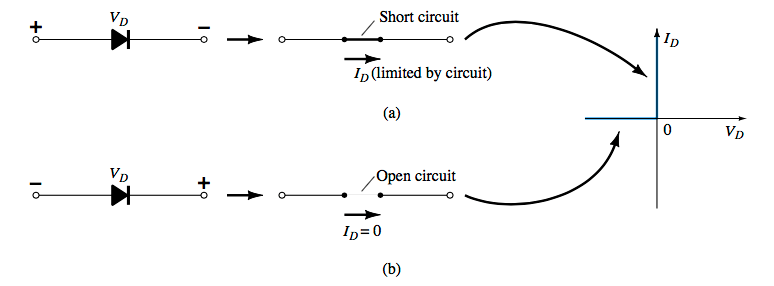
\includegraphics[height = 5cm, width = 16.5cm]{3.png}
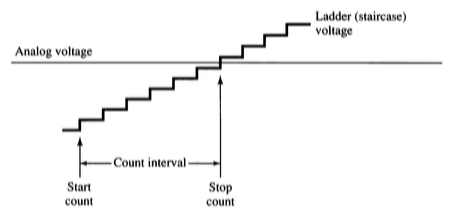
\includegraphics[height = 4cm, width = 16.5cm]{4.png}
\centering \linebreak \linebreak {\small Figure 1.1: Analog-to-digital conversion using ladder network: (a) logic diagram; (b) waveform.}
\end{figure}